%!TEX program = xelatex
% Note: this template must be compiled with XeLaTeX rather than PDFLaTeX
% due to the custom fonts used. The line above should ensure this happens
% automatically, but if it doesn't, your LaTeX editor should have a simple toggle
% to switch to using XeLaTeX.

\documentclass[
  aspectratio=169, % Uncomment to use an aspect ratio of 16:9 (160 mm by 90 mm)
  %aspectratio=43, % Uncomment to use an aspect ratio of 4:3 (128mm by 96mm)
  t, % Top align all slide content by default
  onlytextwidth, % Typeset content in columns at text width
  10pt, % Default font size, use 10pt for the 16:9 aspect ratio and 8pt for the 4:3 aspect ratio
]{beamer}

\usepackage{../../ImperialTheme/beamer/beamerthemeImperial} % Use the Imperial theme

\def\imagefolder{../../ImperialTheme/beamer/Images}
\def\Rey{\text{Re}}
\title{Several things} % Presentation title to appear on the title slide and left footers

\subtitle{} % Presentation subtitle to appear on the title slide

\author{Víctor Ballester} % Author name(s) to appear on the title slide

\date{\today} % Presentation date to appear on the title slide and right footers

\begin{document}

\begingroup
\setbeamercolor{background canvas}{bg=ICLLightGrey} % Slide background color
\setbeamercolor{title page title}{fg=ICLBlue} % Title text color
\setbeamercolor{title page subtitle}{fg=ICLBlue} % Subtitle text color
\setbeamercolor{author}{fg=ICLBlue} % Author(s) text color
\setbeamercolor{date}{fg=ICLBlue} % Date text color
\setbeamertemplate{title page}[logo]{\imagefolder/ICL_Logo_Blue.pdf} % Imperial logo color, use 'ICL_Logo_White.pdf' for white and 'ICL_Logo_Blue.pdf' for blue
\frame[plain, s]{\titlepage} % Output the title page with no footer ('plain') and vertically distributed text ('s')
\endgroup

\begin{frame}
	\frametitle{Reminder}
	\centering

	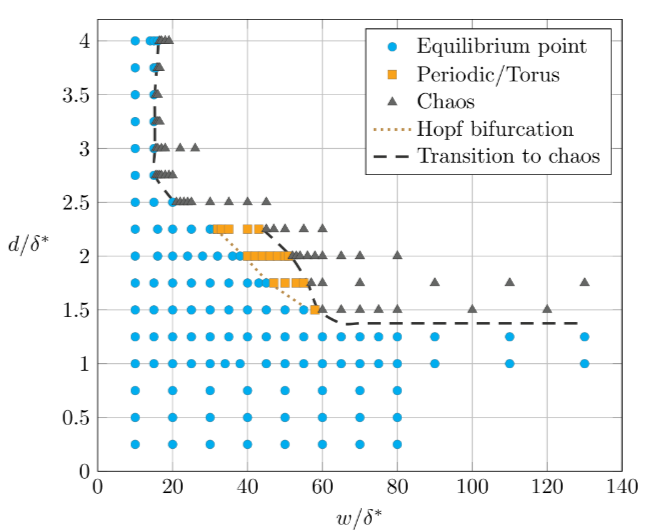
\includegraphics[width=0.5\linewidth]{Images/stabilitycurve.png}
\end{frame}
\begin{frame}
	\frametitle{Homework}
	\begin{itemize}
		\item Interpolating the solution at $d=3$ and $w=15.5$ (not equilibria) into the geometry of $d=3$ and $w=15$ and running the simulation, the solution converges to the same equilibrium point.
		\item I have the feeling that the attractor that we were observing starting around 15.5 it might be another Hopf bifurcation.
	\end{itemize}

\end{frame}
\begin{frame}
	\frametitle{$d=3$ and $w=18$ return map}
	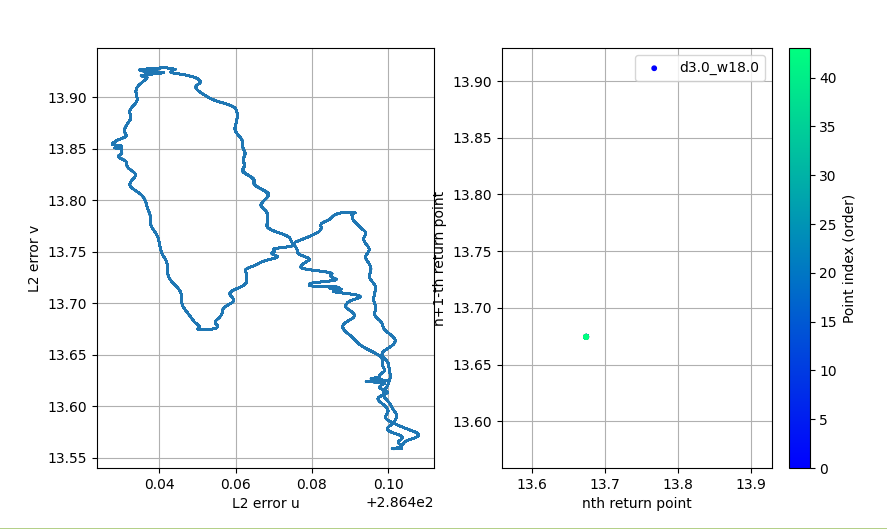
\includegraphics[width=0.8\linewidth]{Images/returnmapd3w18.png}
  
\end{frame}
\begin{frame}
	\frametitle{$d=3$ and $w=18$ return map}
	
\includegraphics[width=\linewidth]{Images/ud3w18.png}  
\end{frame}
\begin{frame}
	\frametitle{$d=3$ and $w=22$ return map}
	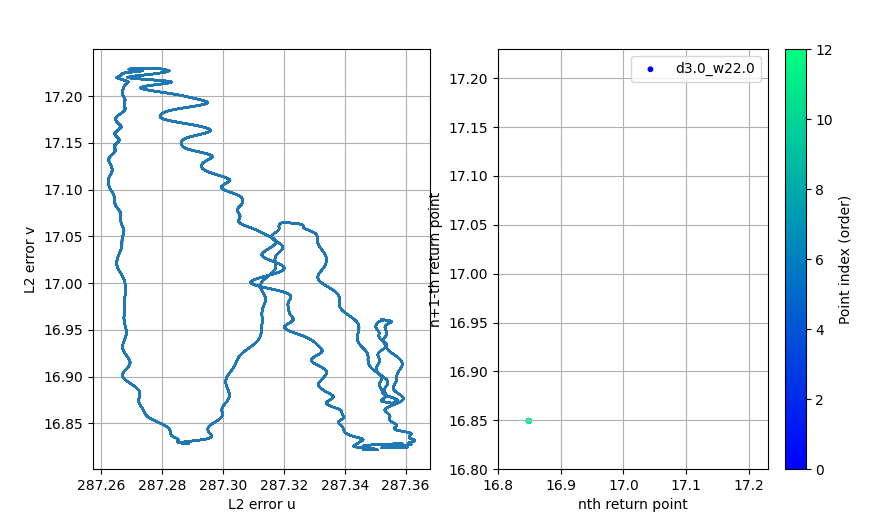
\includegraphics[width=0.8\linewidth]{Images/returnmapd3w22.png}
  
\end{frame}
\begin{frame}
	\frametitle{But $d=3$ and $w=16$ doesn't exhibit this behaviour... Why?}
	\includegraphics[width=0.4\linewidth]{Images/returnmapd3w16.png}
\end{frame}
\begin{frame}
	\frametitle{But $d=3$ and $w=16$ doesn't exhibit this behaviour... Why?}
	
\includegraphics[width=\linewidth]{Images/ud3w16.png}
	\begin{itemize}
	  \item Looks very similar to the previous one at $w=18$.
	\item Numerical issue (e.g. SVV, etc) or physical?
	\end{itemize}
\end{frame}
\begin{frame}
	\frametitle{Edge state at $d=3$ and $w=17$}
	\begin{columns}[T] % [T] ensures correct vertical alignment
		\begin{column}{0.45\linewidth} % Left column
			\begin{itemize}
				\item We choose the L2 norm in the domain as a measure of the amplitude of the perturbation.
				\item Difference between initial conditions:\\
				      $|\|{u_\text{div}\|}_2-\|{u_\text{conv}\|}_2|\sim 4 \cdot 10^{-9}$\\
				      $|\|{v_\text{div}\|}_2-\|{v_\text{conv}\|}_2|\sim 1 \cdot 10^{-10}$
				\item I have the feeling that the unstable state, is just pumping vortices ``differently" from the stable one.
			\end{itemize}
		\end{column}
		\begin{column}{0.54\linewidth} % Left column
			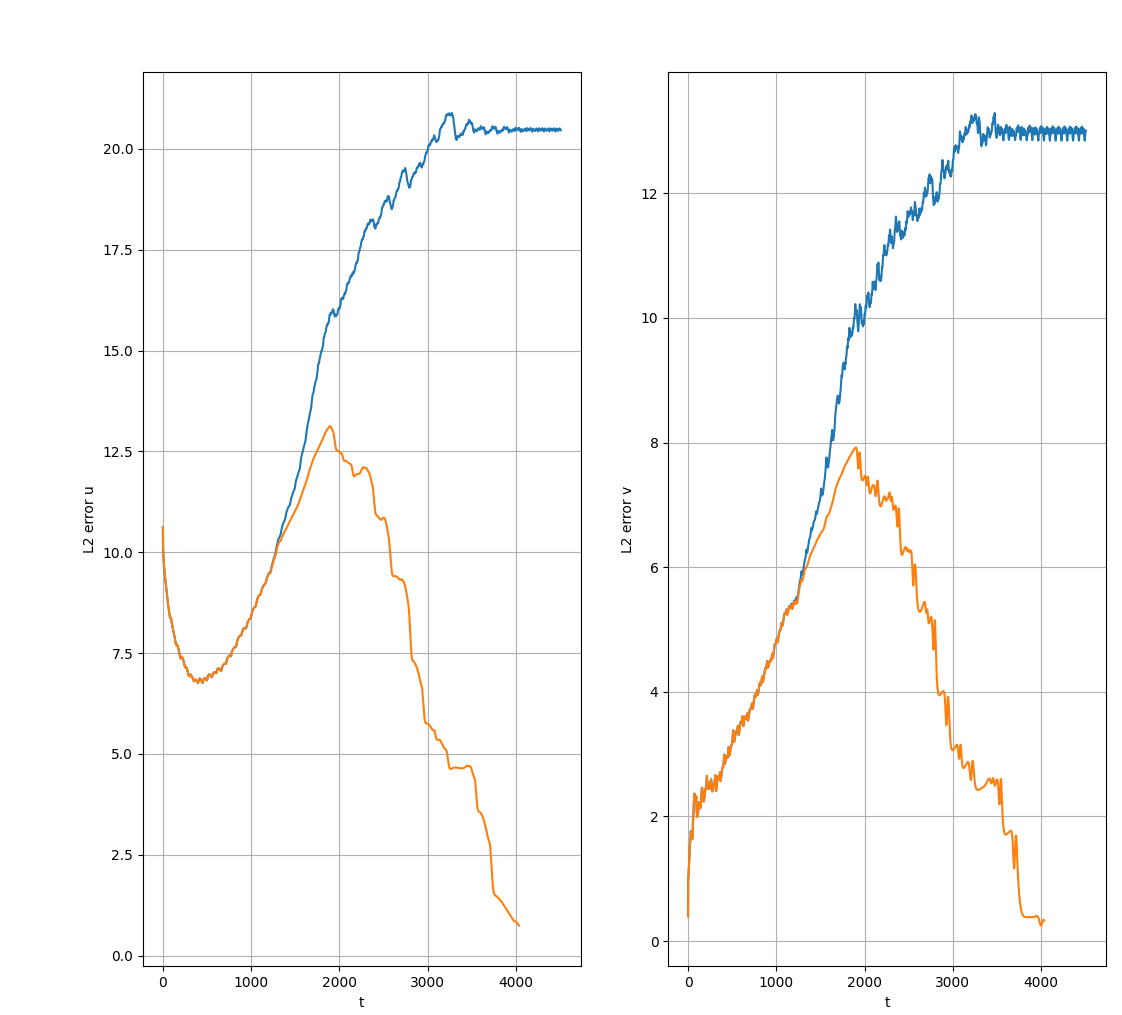
\includegraphics[width=\linewidth]{Images/edgestateEnergy.png}
		\end{column}
	\end{columns}
\end{frame}
\begin{frame}
	\frametitle{Hopf bifurcation amplitude}
	\begin{columns}[T] % [T] ensures correct vertical alignment
		\begin{column}{0.59\linewidth} % Left column
			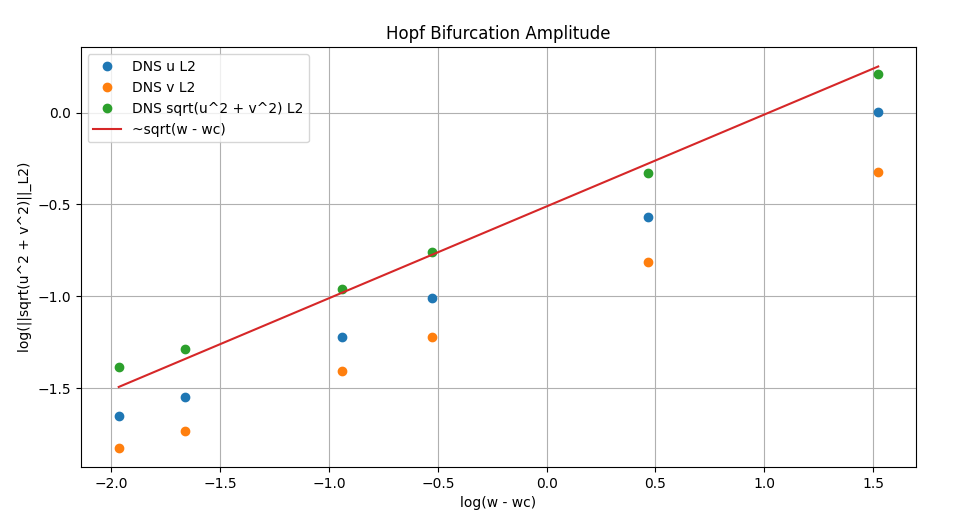
\includegraphics[width=\linewidth]{Images/hopfamplitude.png}
		\end{column}
		\begin{column}{0.39\linewidth} % Left column
			\begin{itemize}
				\item Any amplitude needs to follow $A(w)\sim \sqrt{w-w_c}$
				\item $w_c\in (25.41,25.42)$
				\item Data from $w\in\{25.55,25.6,25.8,26,27,30\}$:
				\item At $w=35$ we already have a torus.
			\end{itemize}
		\end{column}
	\end{columns}
\end{frame}
\begin{frame}
	\frametitle{Edge state at $d=3$ and $w=30$}
	\begin{itemize}
		\item Periodic Orbit, projected to the new system $\|{u}\|_2$ vs $\|{v}\|_2$.
	\end{itemize}
	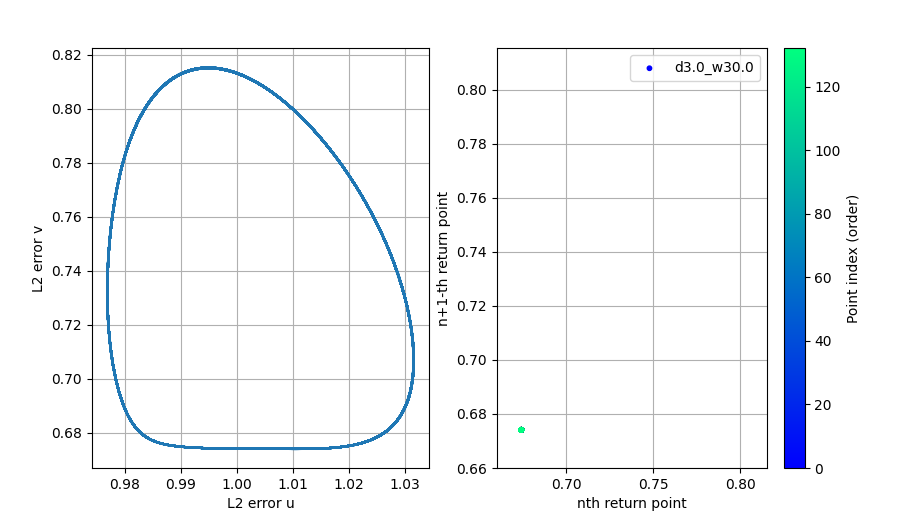
\includegraphics[width=0.8\linewidth]{Images/returnd3_w30.png}
\end{frame}
\begin{frame}
	\frametitle{Edge state at $d=3$ and $w=35$}
	\begin{itemize}
		\item  TORUSSSS!!!! 
		\item From Global stability analysis, we found two unstable modes with different frequencies:
		      \begin{itemize}
			      \item $\sigma=0.012835, \omega = 0.21905$
			      \item $\sigma=0.005983, \omega = 0.26979$
		      \end{itemize}
		      Both modes look very very similar:
		\item Reminder. TS waves freq around the gap: $\sim 0.08$	
	\end{itemize}
	
\includegraphics[width=0.5\linewidth]{Images/globalmoded3w35_1.png}
	
\includegraphics[width=0.5\linewidth]{Images/gloablmoded3w35_2.png}
\end{frame}
\begin{frame}
	\frametitle{Edge state at $d=3$ and $w=35$ return map?}
	\begin{itemize}
	  \item Energy doesn't have any clear distinguishable shape. Why? I think because the two frequencies of the unstable modes couple and propagate the energy to other frequencies exciting the TS modes. This is NOT a transient phenomenon, it is always like this.
	\end{itemize}
	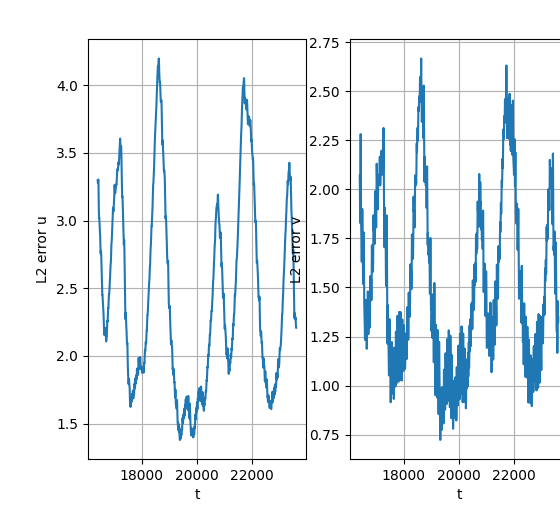
\includegraphics[width=0.4\linewidth]{Images/energyd3w35.png}
\end{frame}
\begin{frame}
	\frametitle{Edge state at $d=3$ and $w=35$ return map?}
	\begin{itemize}
	  \item Energy doesn't have any clear distinguishable shape. Why? I think because the two frequencies of the unstable modes couple and propagate to other energies exciting the TS modes. This is NOT a transient phenomenon, it is always like this.
	\end{itemize}
	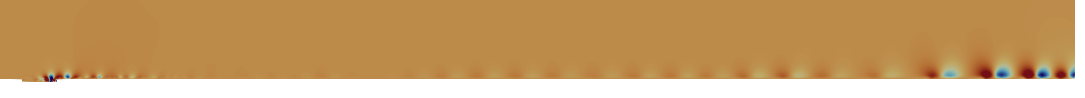
\includegraphics[width=0.9\linewidth]{Images/modesexcitingTSd3w35.png}
\end{frame}
\begin{frame}
	\frametitle{Edge state at $d=3$ and $w=35$ return map?}
	\begin{itemize}
	  \item If we try to do the return map ($u$ vs $v$) very locally in a point just above the gap, we see:
	 \item Of course the shape of the scatter plot in the return maps depends on the point we choose.
	\end{itemize}
	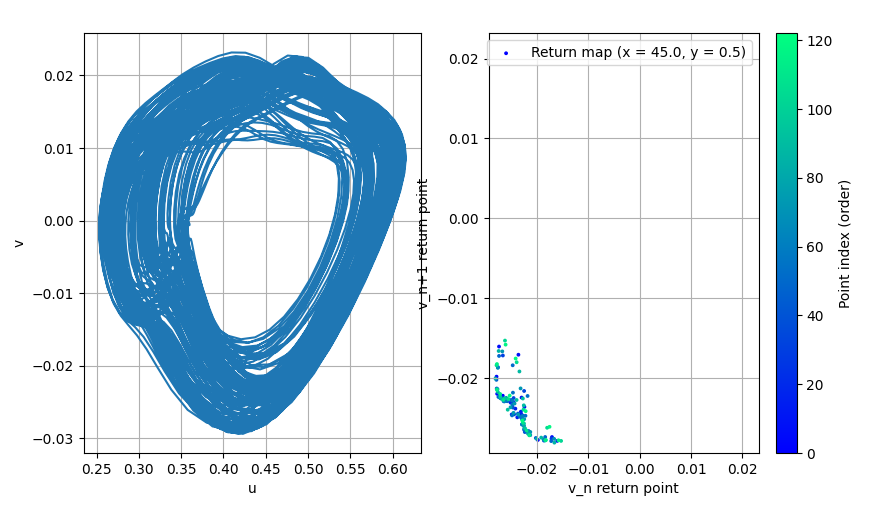
\includegraphics[width=0.8\linewidth]{Images/returnmapd3w35_point1.png}
\end{frame}\end{document}
